\documentclass[border=10pt]{standalone}
\usepackage[left=25mm,right=25mm,top=25mm,bottom=25mm]{geometry}
\usepackage[utf8]{inputenc}
\usepackage[T1]{fontenc}
\usepackage{times}
\usepackage{geometry}
\usepackage{amsmath}
\usepackage{amssymb}
\usepackage{mathrsfs}
\usepackage{amsfonts}
\usepackage{amsthm}
\usepackage{lipsum}
\usepackage{amscd}
\usepackage{graphicx}
\usepackage{fancyhdr}
\usepackage{textcomp}
\usepackage{txfonts}
\usepackage[all]{xy}
\usepackage{paralist}
\usepackage[colorlinks=true]{hyperref}
\usepackage{array}
\usepackage{tikz}
\usepackage{slashed}
\usepackage{pdfpages}
\usepackage{cite}
\usepackage{url}
\usepackage{amsmath,amsfonts,amssymb}
\usepackage{tikz}
\usetikzlibrary{automata,positioning}
\usepackage{listings}
\usepackage{multirow}
\usepackage{color}

\begin{document}

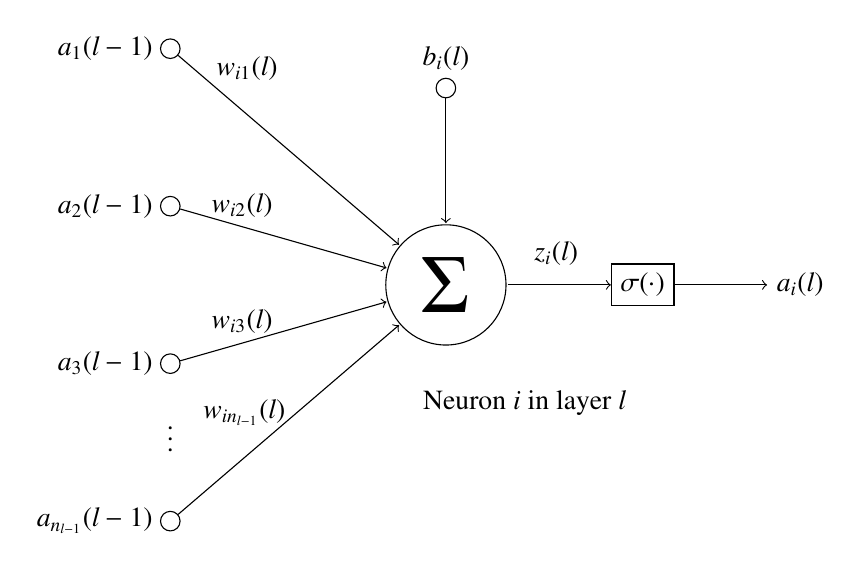
\begin{tikzpicture}
\path
(0,0)     node[circle,draw,scale=3,inner sep=2pt] (S) {$\Sigma$}
+(0,2.5) node[circle,draw,inner sep=2.5pt] (b) {} node[above=1mm] {$b_i(l)$}
+(-3.5,3)  node[circle,draw,inner sep=2.5pt]  (x1) {} node[left=1mm] {$a_1(l-1)$}
+(-3.5,1)    node[circle,draw,inner sep=2.5pt]  (x2) {} node[left=1mm]{$a_2(l-1)$}
+(-3.5,-2.25) node[anchor=south] (dots) {$\vdots$}
+(-3.5,-1) node[circle,draw,inner sep=2.5pt]  (x3) {} node[left=1mm]{$a_3(l-1)$}
+(-3.5,-3) node[circle,draw,inner sep=2.5pt]  (x4) {} node[left=1mm]{$a_{n_{l-1}}(l-1)$}
(2.5,0)    node[draw] (g) {$\sigma(\cdot)$} 
+(0:2)  node[]  (y1) {$a_i(l)$};

\node[] at (1,-1.5) {Neuron $i$ in layer $l$}; 

\draw[->] (S)--(g);
\draw[->] (b)--(S);
\draw[->] (g.east)--(y1) node[pos=.6,above]{};
\draw[->] (x1)--(S) node[pos=.3,above,label={[xshift=1, yshift=1]$w_{i1}(l)$}]{};
\draw[->] (x2)--(S) node[pos=.3,above]{$w_{i2}(l)$};
\draw[->] (x3)--(S) node[pos=.3,above]{$w_{i3}(l)$};
\draw[->] (x4)--(S) node[pos=.3,above,label={[xshift=0, yshift=1]$w_{in_{l-1}}(l)$}]{};
\node[] at (1.4,0.4) {$z_i(l)$};
% \draw[blue] (1,0) circle(2);
\end{tikzpicture}



\end{document}

